% Options for packages loaded elsewhere
\PassOptionsToPackage{unicode}{hyperref}
\PassOptionsToPackage{hyphens}{url}
\PassOptionsToPackage{dvipsnames,svgnames,x11names}{xcolor}
%
\documentclass[
  letterpaper,
  DIV=11,
  numbers=noendperiod]{scrartcl}

\usepackage{amsmath,amssymb}
\usepackage{setspace}
\usepackage{iftex}
\ifPDFTeX
  \usepackage[T1]{fontenc}
  \usepackage[utf8]{inputenc}
  \usepackage{textcomp} % provide euro and other symbols
\else % if luatex or xetex
  \usepackage{unicode-math}
  \defaultfontfeatures{Scale=MatchLowercase}
  \defaultfontfeatures[\rmfamily]{Ligatures=TeX,Scale=1}
\fi
\usepackage{lmodern}
\ifPDFTeX\else  
    % xetex/luatex font selection
\fi
% Use upquote if available, for straight quotes in verbatim environments
\IfFileExists{upquote.sty}{\usepackage{upquote}}{}
\IfFileExists{microtype.sty}{% use microtype if available
  \usepackage[]{microtype}
  \UseMicrotypeSet[protrusion]{basicmath} % disable protrusion for tt fonts
}{}
\makeatletter
\@ifundefined{KOMAClassName}{% if non-KOMA class
  \IfFileExists{parskip.sty}{%
    \usepackage{parskip}
  }{% else
    \setlength{\parindent}{0pt}
    \setlength{\parskip}{6pt plus 2pt minus 1pt}}
}{% if KOMA class
  \KOMAoptions{parskip=half}}
\makeatother
\usepackage{xcolor}
\setlength{\emergencystretch}{3em} % prevent overfull lines
\setcounter{secnumdepth}{-\maxdimen} % remove section numbering
% Make \paragraph and \subparagraph free-standing
\ifx\paragraph\undefined\else
  \let\oldparagraph\paragraph
  \renewcommand{\paragraph}[1]{\oldparagraph{#1}\mbox{}}
\fi
\ifx\subparagraph\undefined\else
  \let\oldsubparagraph\subparagraph
  \renewcommand{\subparagraph}[1]{\oldsubparagraph{#1}\mbox{}}
\fi

\usepackage{color}
\usepackage{fancyvrb}
\newcommand{\VerbBar}{|}
\newcommand{\VERB}{\Verb[commandchars=\\\{\}]}
\DefineVerbatimEnvironment{Highlighting}{Verbatim}{commandchars=\\\{\}}
% Add ',fontsize=\small' for more characters per line
\usepackage{framed}
\definecolor{shadecolor}{RGB}{241,243,245}
\newenvironment{Shaded}{\begin{snugshade}}{\end{snugshade}}
\newcommand{\AlertTok}[1]{\textcolor[rgb]{0.68,0.00,0.00}{#1}}
\newcommand{\AnnotationTok}[1]{\textcolor[rgb]{0.37,0.37,0.37}{#1}}
\newcommand{\AttributeTok}[1]{\textcolor[rgb]{0.40,0.45,0.13}{#1}}
\newcommand{\BaseNTok}[1]{\textcolor[rgb]{0.68,0.00,0.00}{#1}}
\newcommand{\BuiltInTok}[1]{\textcolor[rgb]{0.00,0.23,0.31}{#1}}
\newcommand{\CharTok}[1]{\textcolor[rgb]{0.13,0.47,0.30}{#1}}
\newcommand{\CommentTok}[1]{\textcolor[rgb]{0.37,0.37,0.37}{#1}}
\newcommand{\CommentVarTok}[1]{\textcolor[rgb]{0.37,0.37,0.37}{\textit{#1}}}
\newcommand{\ConstantTok}[1]{\textcolor[rgb]{0.56,0.35,0.01}{#1}}
\newcommand{\ControlFlowTok}[1]{\textcolor[rgb]{0.00,0.23,0.31}{#1}}
\newcommand{\DataTypeTok}[1]{\textcolor[rgb]{0.68,0.00,0.00}{#1}}
\newcommand{\DecValTok}[1]{\textcolor[rgb]{0.68,0.00,0.00}{#1}}
\newcommand{\DocumentationTok}[1]{\textcolor[rgb]{0.37,0.37,0.37}{\textit{#1}}}
\newcommand{\ErrorTok}[1]{\textcolor[rgb]{0.68,0.00,0.00}{#1}}
\newcommand{\ExtensionTok}[1]{\textcolor[rgb]{0.00,0.23,0.31}{#1}}
\newcommand{\FloatTok}[1]{\textcolor[rgb]{0.68,0.00,0.00}{#1}}
\newcommand{\FunctionTok}[1]{\textcolor[rgb]{0.28,0.35,0.67}{#1}}
\newcommand{\ImportTok}[1]{\textcolor[rgb]{0.00,0.46,0.62}{#1}}
\newcommand{\InformationTok}[1]{\textcolor[rgb]{0.37,0.37,0.37}{#1}}
\newcommand{\KeywordTok}[1]{\textcolor[rgb]{0.00,0.23,0.31}{#1}}
\newcommand{\NormalTok}[1]{\textcolor[rgb]{0.00,0.23,0.31}{#1}}
\newcommand{\OperatorTok}[1]{\textcolor[rgb]{0.37,0.37,0.37}{#1}}
\newcommand{\OtherTok}[1]{\textcolor[rgb]{0.00,0.23,0.31}{#1}}
\newcommand{\PreprocessorTok}[1]{\textcolor[rgb]{0.68,0.00,0.00}{#1}}
\newcommand{\RegionMarkerTok}[1]{\textcolor[rgb]{0.00,0.23,0.31}{#1}}
\newcommand{\SpecialCharTok}[1]{\textcolor[rgb]{0.37,0.37,0.37}{#1}}
\newcommand{\SpecialStringTok}[1]{\textcolor[rgb]{0.13,0.47,0.30}{#1}}
\newcommand{\StringTok}[1]{\textcolor[rgb]{0.13,0.47,0.30}{#1}}
\newcommand{\VariableTok}[1]{\textcolor[rgb]{0.07,0.07,0.07}{#1}}
\newcommand{\VerbatimStringTok}[1]{\textcolor[rgb]{0.13,0.47,0.30}{#1}}
\newcommand{\WarningTok}[1]{\textcolor[rgb]{0.37,0.37,0.37}{\textit{#1}}}

\providecommand{\tightlist}{%
  \setlength{\itemsep}{0pt}\setlength{\parskip}{0pt}}\usepackage{longtable,booktabs,array}
\usepackage{calc} % for calculating minipage widths
% Correct order of tables after \paragraph or \subparagraph
\usepackage{etoolbox}
\makeatletter
\patchcmd\longtable{\par}{\if@noskipsec\mbox{}\fi\par}{}{}
\makeatother
% Allow footnotes in longtable head/foot
\IfFileExists{footnotehyper.sty}{\usepackage{footnotehyper}}{\usepackage{footnote}}
\makesavenoteenv{longtable}
\usepackage{graphicx}
\makeatletter
\def\maxwidth{\ifdim\Gin@nat@width>\linewidth\linewidth\else\Gin@nat@width\fi}
\def\maxheight{\ifdim\Gin@nat@height>\textheight\textheight\else\Gin@nat@height\fi}
\makeatother
% Scale images if necessary, so that they will not overflow the page
% margins by default, and it is still possible to overwrite the defaults
% using explicit options in \includegraphics[width, height, ...]{}
\setkeys{Gin}{width=\maxwidth,height=\maxheight,keepaspectratio}
% Set default figure placement to htbp
\makeatletter
\def\fps@figure{htbp}
\makeatother
\newlength{\cslhangindent}
\setlength{\cslhangindent}{1.5em}
\newlength{\csllabelwidth}
\setlength{\csllabelwidth}{3em}
\newlength{\cslentryspacingunit} % times entry-spacing
\setlength{\cslentryspacingunit}{\parskip}
\newenvironment{CSLReferences}[2] % #1 hanging-ident, #2 entry spacing
 {% don't indent paragraphs
  \setlength{\parindent}{0pt}
  % turn on hanging indent if param 1 is 1
  \ifodd #1
  \let\oldpar\par
  \def\par{\hangindent=\cslhangindent\oldpar}
  \fi
  % set entry spacing
  \setlength{\parskip}{#2\cslentryspacingunit}
 }%
 {}
\usepackage{calc}
\newcommand{\CSLBlock}[1]{#1\hfill\break}
\newcommand{\CSLLeftMargin}[1]{\parbox[t]{\csllabelwidth}{#1}}
\newcommand{\CSLRightInline}[1]{\parbox[t]{\linewidth - \csllabelwidth}{#1}\break}
\newcommand{\CSLIndent}[1]{\hspace{\cslhangindent}#1}

\usepackage{booktabs}
\usepackage{longtable}
\usepackage{array}
\usepackage{multirow}
\usepackage{wrapfig}
\usepackage{float}
\usepackage{colortbl}
\usepackage{pdflscape}
\usepackage{tabu}
\usepackage{threeparttable}
\usepackage{threeparttablex}
\usepackage[normalem]{ulem}
\usepackage{makecell}
\usepackage{xcolor}
\KOMAoption{captions}{tableheading}
\makeatletter
\makeatother
\makeatletter
\makeatother
\makeatletter
\@ifpackageloaded{caption}{}{\usepackage{caption}}
\AtBeginDocument{%
\ifdefined\contentsname
  \renewcommand*\contentsname{Table of contents}
\else
  \newcommand\contentsname{Table of contents}
\fi
\ifdefined\listfigurename
  \renewcommand*\listfigurename{List of Figures}
\else
  \newcommand\listfigurename{List of Figures}
\fi
\ifdefined\listtablename
  \renewcommand*\listtablename{List of Tables}
\else
  \newcommand\listtablename{List of Tables}
\fi
\ifdefined\figurename
  \renewcommand*\figurename{Figure}
\else
  \newcommand\figurename{Figure}
\fi
\ifdefined\tablename
  \renewcommand*\tablename{Table}
\else
  \newcommand\tablename{Table}
\fi
}
\@ifpackageloaded{float}{}{\usepackage{float}}
\floatstyle{ruled}
\@ifundefined{c@chapter}{\newfloat{codelisting}{h}{lop}}{\newfloat{codelisting}{h}{lop}[chapter]}
\floatname{codelisting}{Listing}
\newcommand*\listoflistings{\listof{codelisting}{List of Listings}}
\makeatother
\makeatletter
\@ifpackageloaded{caption}{}{\usepackage{caption}}
\@ifpackageloaded{subcaption}{}{\usepackage{subcaption}}
\makeatother
\makeatletter
\@ifpackageloaded{tcolorbox}{}{\usepackage[skins,breakable]{tcolorbox}}
\makeatother
\makeatletter
\@ifundefined{shadecolor}{\definecolor{shadecolor}{rgb}{.97, .97, .97}}
\makeatother
\makeatletter
\makeatother
\makeatletter
\makeatother
\ifLuaTeX
  \usepackage{selnolig}  % disable illegal ligatures
\fi
\IfFileExists{bookmark.sty}{\usepackage{bookmark}}{\usepackage{hyperref}}
\IfFileExists{xurl.sty}{\usepackage{xurl}}{} % add URL line breaks if available
\urlstyle{same} % disable monospaced font for URLs
\hypersetup{
  pdftitle={Causal inference is not a statistical problem},
  pdfauthor={Lucy D'Agostino McGowan; Travis Gerke; Malcolm Barrett},
  colorlinks=true,
  linkcolor={blue},
  filecolor={Maroon},
  citecolor={Blue},
  urlcolor={Blue},
  pdfcreator={LaTeX via pandoc}}

\title{Causal inference is not a statistical problem}
\author{Lucy D'Agostino McGowan \and Travis Gerke \and Malcolm Barrett}
\date{}

\begin{document}
\maketitle
\ifdefined\Shaded\renewenvironment{Shaded}{\begin{tcolorbox}[boxrule=0pt, sharp corners, interior hidden, breakable, enhanced, borderline west={3pt}{0pt}{shadecolor}, frame hidden]}{\end{tcolorbox}}\fi

\setstretch{2}
\hypertarget{abstract}{%
\subsection{Abstract}\label{abstract}}

This paper introduces a collection of four data sets, similar to
Anscombe's Quartet, that aim to highlight the challenges involved when
estimating causal effects. Each of the four data sets is generated based
on a distinct causal mechanism: the first consists of a collider, the
second involves a confounder, the third involves a mediator, and the
fourth involves the induction of M-Bias by an included factor. The paper
contains a mathematical summary of each data set and directed acyclic
graphs depicting the relationships between the variables. Even though
the statistical summaries and visualizations for each data set are
identical, the true causal effect differs. Correctly estimating the
effect requires knowledge of the data-generating mechanism. These
example data sets can help practitioners gain a better understanding of
the assumptions underlying causal inference methods and emphasize the
importance of gathering more information beyond what can be obtained
from statistical tools alone. The paper also includes R code for
reproducing all figures and provides access to the data sets through an
R package named quartets.

\hypertarget{introduction}{%
\subsection{Introduction}\label{introduction}}

Anscombe's Quartet is a set of four data sets with the same summary
statistics (means, variances, correlations, and linear regression fits)
but exhibit different distributions and relationships when plotted on a
graph (Anscombe 1973). Often used to teach introductory statistics
courses, Anscombe created the quartet to illustrate the importance of
visualizing data before drawing conclusions based on statistical
analyses alone. Here, we propose a different quartet, where statistical
summaries do not provide insight into the underlying mechanism, but even
visualizations do not solve the issue. In these examples, to correctly
capture the relationship between the available factors, the research
needs to understand or make assumptions about the data-generating
mechanism. This proposed quartet can help practitioners better
understand the assumptions underlying causal inference methods, further
driving home the point that we require more information than can be
gleaned from statistical tools alone to estimate causal effects
accurately.

The data generated to create the figures displayed here are available in
an R package titled \texttt{quartets} (D'Agostino McGowan 2023).

\hypertarget{causal-inference-primer}{%
\subsection{Causal inference primer}\label{causal-inference-primer}}

In causal inference, we often try to estimate the effect of some
exposure, \(X\), on some outcome \(Y\). One framework to think through
this problem is the ``potential outcomes'' framework (Rubin 1974). Here,
you can imagine each individual has a set of potential outcomes under
each possible exposure value. For example, if there are two levels of
exposure (exposed: 1 and unexposed: 0), we could have the potential
outcome under exposure (\(Y(1)\)) and the potential outcome under no
exposure (\(Y(0)\)) and look at the difference between these,
\(Y(1) - Y(0)\) to understand the impact on the exposure on the outcome,
\(Y\). Of course, at any moment, only one of these potential outcomes is
observable: the potential outcome corresponding to the exposure the
individual \emph{actually} experienced. Under certain assumptions, we
can borrow information from individuals who have received different
exposures to compare the average difference between their observed
outcomes. We assume that one individual's exposure does not impact the
outcome of any other individual. We also assume that everyone has some
chance of having each level of the exposure. And finally, we assume that
the exposure the person receives has nothing to do with how we think it
will affect them after adjusting for a set of observed covariates. In
other words, the potential outcomes are independent of the exposure
value the individual experienced given the covariate(s) \emph{that we
adjust for} in our modeling process. Of course, the entire point of
causal inference is because we believe an exposure may cause an outcome;
this assumption relates to the \emph{assignment} to a specific exposure
value. The easiest way to think about this is when the exposure is
\emph{randomly assigned} to each individual, ensuring this assumption is
true without needing to adjust for any other factors. In non-randomized
settings, we must likely adjust for other factors to satisfy this
independence. The problem is identifying which factors are required, as
adjusting for all observed factors may not be appropriate (and may even
give you the wrong effect). The purpose of this paper is to focus on the
observed covariates, \(Z\). Given you have three variables, an exposure,
\(X\), an outcome, \(Y\), and some measured factor, \(Z\), how do you
decide whether you should estimate the average treatment effect
adjusting for \(Z\)?

\hypertarget{methods}{%
\subsection{Methods}\label{methods}}

We propose the following four data generation mechanisms, summarized by
the equations below and the directed acyclic graphs displayed in
Figure~\ref{fig-1}. Here, \(X\) is presumed to be some continuous
exposure of interest, \(Y\) a continuous outcome, and \(Z\) a known,
measured factor. The M-Bias equation includes two additional, unmeasured
factors, \(U_1\) and \(U_2\).

\begin{enumerate}
\def\labelenumi{(\arabic{enumi})}
\tightlist
\item
  Collider:
\end{enumerate}

\begin{equation}\protect\hypertarget{eq-col}{}{
\begin{split}
X &\sim N(0, 1)\\
Y &= X + \varepsilon_y, \textrm{ }\varepsilon_y\sim N(0, 1)\\
Z &=  0.45X + 0.77 Y + \varepsilon_z, \textrm{ }\varepsilon_z \sim N(0,1)
\end{split}
}\label{eq-col}\end{equation}

\begin{enumerate}
\def\labelenumi{(\arabic{enumi})}
\setcounter{enumi}{1}
\tightlist
\item
  Confounder:
\end{enumerate}

\begin{equation}\protect\hypertarget{eq-conf}{}{
\begin{split}
Z &\sim N(0, 1)\\
X &= Z + \varepsilon_x,\textrm{ }\varepsilon_x\sim N(0, 1)\\
Y &=  0.5X + Z + \varepsilon_y, \textrm{ }\varepsilon_y\sim N(0, 1)
\end{split}
}\label{eq-conf}\end{equation}

\begin{enumerate}
\def\labelenumi{(\arabic{enumi})}
\setcounter{enumi}{2}
\tightlist
\item
  Mediator:
\end{enumerate}

\begin{equation}\protect\hypertarget{eq-med}{}{
\begin{split}
X &\sim N(0, 1)\\
Z &= X + \varepsilon_z, \textrm{ }\varepsilon_z\sim N(0, 1)\\
Y &=  Z + \varepsilon_y, \textrm{ }\varepsilon_y\sim N(0, 1)
\end{split}
}\label{eq-med}\end{equation}

\begin{enumerate}
\def\labelenumi{(\arabic{enumi})}
\setcounter{enumi}{3}
\tightlist
\item
  M-Bias:
\end{enumerate}

\begin{equation}\protect\hypertarget{eq-mbias}{}{
\begin{split}
U_1 &\sim N(0, 1)\\
U_2 &\sim N(0, 1)\\
Z &= 8 U_1 + U_2 + \varepsilon_z, \textrm{ }\varepsilon_z\sim N(0, 1)\\
X &=  U_1 + \varepsilon_x, \textrm{ }\varepsilon_x\sim N(0, 1)\\
Y &=  X + U_2 + \varepsilon_y, \textrm{ }\varepsilon_y\sim N(0, 1)
\end{split}
}\label{eq-mbias}\end{equation}

In each of these scenarios, a linear model fit to estimate the
relationship between \(X\) and \(Y\) with no further adjustment will
result in a \(\hat\beta\) coefficient of 1. Or, equivalently, the
estimated average treatment effect (ATE) without adjusting for \(Z\) is
1. The correlation between \(X\) and the additional known factor \(Z\)
is also 0.70.

We have simulated 100 data points from each of the four mechanisms; we
display each in Figure~\ref{fig-2}. This set of figures demonstrates
that despite the very different data-generating mechanisms, there is no
clear way to determine the ``appropriate'' way to model the effect of
the exposure \(X\) and the outcome \(Y\) without additional information.
For example, the unadjusted models are displayed in Figure~\ref{fig-2},
showing a relationship between \(X\) and \(Y\) of 1. The unadjusted
models are the correct causal model for data-generating mechanisms (1)
and (4); however, it overstates the effect of \(X\) for data-generating
mechanism (2) and describes the total effect of \(X\) on \(Y\) for
data-generating mechanism (3), but not the direct effect
(Table~\ref{tbl-1}). Even examining the correlation between \(X\) and
the known factor \(Z\) does not help us determine whether adjusting for
\(Z\) is appropriate, as it is 0.7 in all cases (Table~\ref{tbl-2}). The
four datasets are available in the \texttt{quartets} R package
(D'Agostino McGowan 2023).

\begin{figure}

{\centering 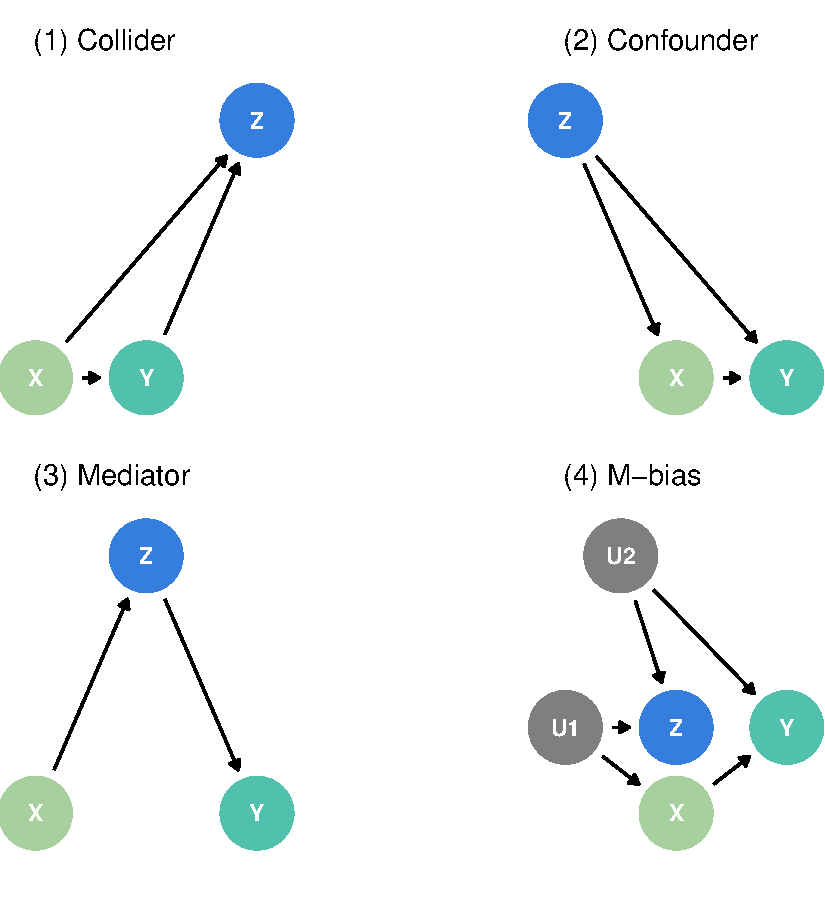
\includegraphics{manuscript_files/figure-pdf/fig-1-1.pdf}

}

\caption{\label{fig-1}Directed Acyclic Graphs describing the four data
generating mechanisms: (1) Collider (2) Confounder (3) Mediator (4)
M-Bias.}

\end{figure}

\begin{figure}

{\centering 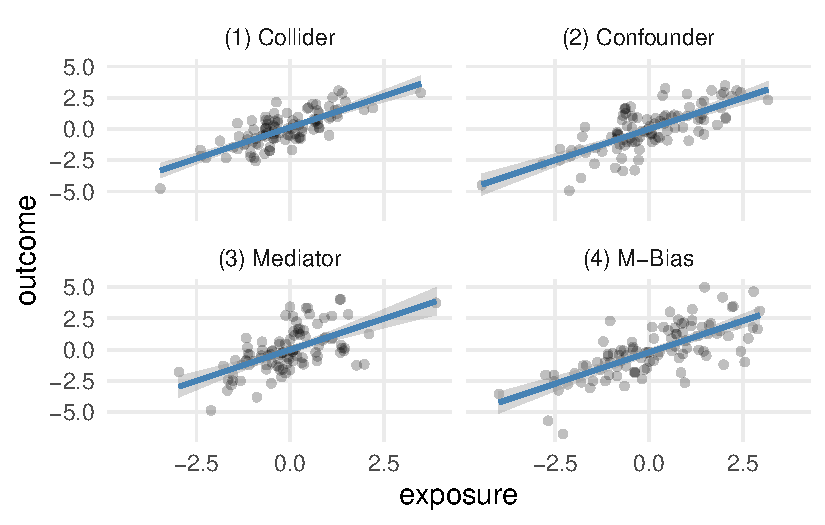
\includegraphics{manuscript_files/figure-pdf/fig-2-1.pdf}

}

\caption{\label{fig-2}100 points generated using the data generating
mechanisms specified (1) Collider (2) Confounder (3) Mediator (4)
M-Bias. The blue line displays a linear regression fit estimating the
relationship between X and Y; in each case, the slope is 1.}

\end{figure}

\hypertarget{tbl-1}{}
\begin{longtable}[]{@{}
  >{\raggedright\arraybackslash}p{(\columnwidth - 4\tabcolsep) * \real{0.3457}}
  >{\raggedright\arraybackslash}p{(\columnwidth - 4\tabcolsep) * \real{0.3457}}
  >{\raggedright\arraybackslash}p{(\columnwidth - 4\tabcolsep) * \real{0.2963}}@{}}
\caption{\label{tbl-1}Correct causal models and causal effects for each
data-generating mechanism. The notation \(X ; Z\) implies that we should
adjust for \(Z\) when estimating the causal effect. In other words, for
the confounder data-generating mechanism and direct effect mediator
model, the potential outcomes are independent of exposure given the
observed covariate \(Z\).}\tabularnewline
\toprule\noalign{}
\begin{minipage}[b]{\linewidth}\raggedright
Data generating mechanism
\end{minipage} & \begin{minipage}[b]{\linewidth}\raggedright
Correct causal model
\end{minipage} & \begin{minipage}[b]{\linewidth}\raggedright
Correct causal effect
\end{minipage} \\
\midrule\noalign{}
\endfirsthead
\toprule\noalign{}
\begin{minipage}[b]{\linewidth}\raggedright
Data generating mechanism
\end{minipage} & \begin{minipage}[b]{\linewidth}\raggedright
Correct causal model
\end{minipage} & \begin{minipage}[b]{\linewidth}\raggedright
Correct causal effect
\end{minipage} \\
\midrule\noalign{}
\endhead
\bottomrule\noalign{}
\endlastfoot
(1) Collider & Y \textasciitilde{} X & 1 \\
(2) Confounder & Y \textasciitilde{} X ; Z & 0.5 \\
(3) Mediator & Direct effect: Y \textasciitilde{} X ; Z

Total Effect: Y \textasciitilde{} X & Direct effect: 0

Total effect: 1 \\
(4) M-Bias & Y \textasciitilde{} X & 1 \\
\end{longtable}

\hypertarget{tbl-2}{}
\begin{table}
\caption{\label{tbl-2}Coefficients for the exposure under each data generating mechanism
depending on the model fit as well as the correlation between \(X\) and
\(Z\). }\tabularnewline

\centering
\begin{tabular}{lrrr}
\toprule
Data generating mechanism & \makecell[c]{ATE\\not adjusting for Z} & \makecell[c]{ATE\\adjusting for Z} & \makecell[c]{Correlation of\\X and Z}\\
\midrule
(1) Collider & 1 & 0.55 & 0.7\\
(2) Confounder & 1 & 0.50 & 0.7\\
(3) Mediator & 1 & 0.00 & 0.7\\
(4) M-Bias & 1 & 0.88 & 0.7\\
\bottomrule
\end{tabular}
\end{table}

\hypertarget{the-solution}{%
\subsection{The Solution}\label{the-solution}}

Here we have demonstrated that when presented with an exposure, outcome,
and some measured factors, statistics alone, whether summary statistics
or data visualizations are insufficient to determine the appropriate
causal estimate. Analysts need additional information about the
data-generating mechanism to draw the correct conclusions. While
knowledge of the data-generating process is necessary to estimate the
right causal effect in each of the cases presented, an analyst can take
steps to make mistakes such as those shown here less likely. The first
is discussing understood mechanisms with content matter experts before
estimating causal effects. Drawing the proposed relationships via causal
diagrams such as the directed acyclic graphs shown in Figure~\ref{fig-1}
before calculating any statistical quantities can help the analyst
ensure they are only adjusting for factors that meet the ``backdoor
criterion,'' that is, adjusting for only factors that close all backdoor
paths between the exposure and outcome of interest (Pearl 2000).

\begin{figure}

\begin{minipage}[t]{0.50\linewidth}

{\centering 

\raisebox{-\height}{

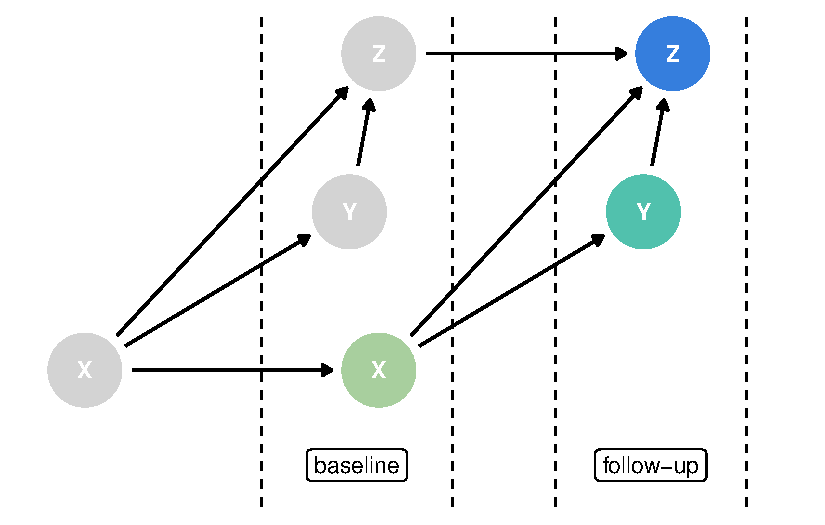
\includegraphics{manuscript_files/figure-pdf/fig-3-1.pdf}

}

}

\subcaption{\label{fig-3-1}Adjusting for \(Z\) as shown here would
induce collider bias.}
\end{minipage}%
%
\begin{minipage}[t]{0.50\linewidth}

{\centering 

\raisebox{-\height}{

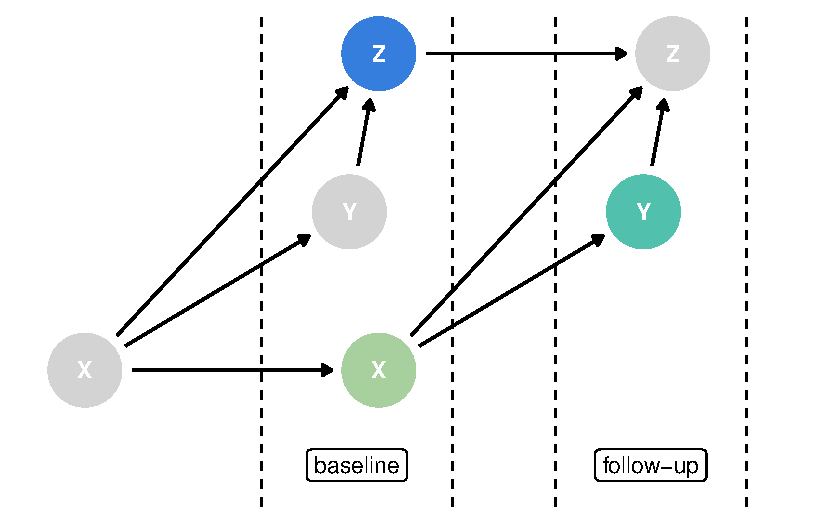
\includegraphics{manuscript_files/figure-pdf/fig-3-2.pdf}

}

}

\subcaption{\label{fig-3-2}Adjusting for this pre-exposure \(Z\) as
shown here would \textbf{not} induce collider bias.}
\end{minipage}%

\caption{\label{fig-3}Time-ordered collider DAG where each factor is
measured twice. \(X\) is the exposure, \(Y\) is the outcome, and \(Z\)
is the measured factor. The highlighted \(Z\) node indicates which time
point is being adjusted for when estimating the average treatment effect
of the highlighted \(X\) on the highlighted \(Y\)}

\end{figure}

Absent subject matter expertise, the analyst can at least consider the
time ordering of the available factors. Fundamental principles of causal
inference dictate that the exposure of interest must precede the outcome
of interest to establish a causal relationship plausibly. In addition,
to account for potential confounding, any covariates adjusted for in the
analysis must precede the exposure in time. Including this additional
timing information would omit the potential for two of the three
misspecified models above (Equation~\ref{eq-col} the ``collider'' and
Equation~\ref{eq-med} the ``mediator'') as the former would demonstrate
that the factor \(Z\) falls after both the exposure and outcome and the
latter would show that the factor \(Z\) falls between the exposure and
the outcome in time. For example, if we drew the second panel of
Figure~\ref{fig-1} (the Collider) as a time-ordered DAG, we would see
something like Figure~\ref{fig-3}. If we carefully adjust only for
factors that are measured pre-exposure, we would not induce the bias we
see in Table~\ref{tbl-2} (Figure~\ref{fig-3-2}). The Causal Quartets
data sets are accompanied by four data sets with time-varying measures
for each factor, \(X\), \(Y\), and \(Z\), generated under the same
data-generating mechanisms. If we adjust for the pre-exposure
measurement of \(Z\), we get the correct causal effect in all scenarios
except M-Bias (Table~\ref{tbl-3}).

\hypertarget{tbl-3}{}
\begin{table}
\caption{\label{tbl-3}Coefficients for the exposure under each data generating mechanism
depending on the model fit as well as the correlation between \(X\) and
\(Z\). }\tabularnewline

\centering
\begin{tabular}{lrrr}
\toprule
Data generating mechanism & \makecell[c]{ATE\\not adjusting for\\pre-exposure Z} & \makecell[c]{ATE\\adjusting for\\pre-exposure Z} & Correct causal effect\\
\midrule
(1) Collider & 1 & 1.00 & 1.0\\
(2) Confounder & 1 & 0.50 & 0.5\\
(3) Mediator & 1 & 1.00 & 1.0\\
(4) M-Bias & 1 & 0.88 & 1.0\\
\bottomrule
\end{tabular}
\end{table}

Adjusting for only pre-exposure factors is widely recommended. The only
exception is when a known confounder is only measured after the exposure
in a particular data analysis, in which case some experts recommend
adjusting for it. Still, even then, caution is advised (Groenwold,
Palmer, and Tilling 2021). Many causal inference methodologists would
recommend conditioning on \emph{all} measured pre-exposure factors
(Rosenbaum 2002; Rubin 2009, 2008; Rubin and Thomas 1996). Including
timing information alone (and thus adjusting for all pre-exposure
factors) does not preclude one from mistakenly fitting the adjusted
model under the fourth data generating mechanism (M-bias), as \(Z\) can
fall temporally before \(X\) and \(Y\) and still induce bias. Some
authors have argued, however, that this strict M-bias (e.g., where
\(U_1\) and \(U_2\) in Equation~\ref{eq-mbias} have no relationship with
each other and \(Z\) has no relationship with \(X\) or \(Y\) other than
via \(U_1\) and \(U_2\)) is very rare in most practical settings (Liu et
al. 2012; Rubin 2009; Gelman 2011). Indeed, even theoretical results
have demonstrated that bias induced by this data-generating mechanism is
sensitive to deviations from this form (Ding and Miratrix 2015).

\hypertarget{discussion}{%
\subsection{Discussion}\label{discussion}}

Anscombe's Quartet has inspired the use of small data sets to
demonstrate key concepts in various data analytic problems. Recent
examples include an extension of the original idea proposed by Anscombe
called the ``Datasaurus Dozen'' (Matejka and Fitzmaurice 2017), an
exploration of varying interaction effects (Rohrer and Arslan 2021), a
quartet of model types fit to the same data that yield the same
performance metrics but fit very different underlying mechanisms
(Biecek, Baniecki, and Krzyznski 2023), and a set of conceptual causal
quartets that highlight the impact of treatment heterogeneity on the
average treatment effect (Gelman, Hullman, and Kennedy 2023). While
similar in name, the conceptual causal quartets differ from what we
present here as they provide excellent insight into how variation in a
treatment effect/treatment heterogeneity can impact an average treatment
effect (by plotting the latent true causal effect). Both sets provide
essential and complementary understanding for data analysis
practitioners.

We have presented four example data sets demonstrating the importance of
understanding the data-generating mechanism when attempting to answer
causal questions. These data indicate that more than statistical
summaries and visualizations are needed to provide insight into the
underlying relationship between the variables. An understanding or
assumption of the data-generating mechanism is required to capture
causal relationships correctly. These examples underscore the
limitations of relying solely on statistical tools in data analyses and
highlight the crucial role of domain-specific knowledge. Moreover, they
emphasize the importance of considering the timing of factors when
deciding what to adjust for.

\hypertarget{references}{%
\subsection{References}\label{references}}

\hypertarget{refs}{}
\begin{CSLReferences}{1}{0}
\leavevmode\vadjust pre{\hypertarget{ref-anscombe1973graphs}{}}%
Anscombe, Francis J. 1973. {``Graphs in Statistical Analysis.''}
\emph{The American Statistician} 27 (1): 17--21.

\leavevmode\vadjust pre{\hypertarget{ref-biecek2023performance}{}}%
Biecek, Przemyslaw, Hubert Baniecki, and Mateusz Krzyznski. 2023.
{``Performance Is Not Enough: A Story of the Rashomon's Quartet.''}
\emph{arXiv Preprint arXiv:2302.13356}.

\leavevmode\vadjust pre{\hypertarget{ref-quartet}{}}%
D'Agostino McGowan, Lucy. 2023. \emph{Quartets: Datasets to Help Teach
Statistics}.

\leavevmode\vadjust pre{\hypertarget{ref-ding2015adjust}{}}%
Ding, Peng, and Luke W Miratrix. 2015. {``To Adjust or Not to Adjust?
Sensitivity Analysis of m-Bias and Butterfly-Bias.''} \emph{Journal of
Causal Inference} 3 (1): 41--57.

\leavevmode\vadjust pre{\hypertarget{ref-gelman2011causality}{}}%
Gelman, Andrew. 2011. {``Causality and Statistical Learning.''}
University of Chicago Press Chicago, IL.

\leavevmode\vadjust pre{\hypertarget{ref-gelman2023causal}{}}%
Gelman, Andrew, Jessica Hullman, and Lauren Kennedy. 2023. {``Causal
Quartets: Different Ways to Attain the Same Average Treatment Effect.''}
\emph{arXiv Preprint arXiv:2302.12878}.

\leavevmode\vadjust pre{\hypertarget{ref-groenwold2021adjust}{}}%
Groenwold, Rolf HH, Tom M Palmer, and Kate Tilling. 2021. {``To Adjust
or Not to Adjust? When a {`Confounder'} Is Only Measured After
Exposure.''} \emph{Epidemiology (Cambridge, Mass.)} 32 (2): 194.

\leavevmode\vadjust pre{\hypertarget{ref-liu2012implications}{}}%
Liu, Wei, M Alan Brookhart, Sebastian Schneeweiss, Xiaojuan Mi, and Soko
Setoguchi. 2012. {``Implications of m Bias in Epidemiologic Studies: A
Simulation Study.''} \emph{American Journal of Epidemiology} 176 (10):
938--48.

\leavevmode\vadjust pre{\hypertarget{ref-matejka2017same}{}}%
Matejka, Justin, and George Fitzmaurice. 2017. {``Same Stats, Different
Graphs: Generating Datasets with Varied Appearance and Identical
Statistics Through Simulated Annealing.''} In \emph{Proceedings of the
2017 CHI Conference on Human Factors in Computing Systems}, 1290--94.

\leavevmode\vadjust pre{\hypertarget{ref-pearl2000causality}{}}%
Pearl, Judea. 2000. \emph{Causality: Models, Reasoning, and Inference}.
Cambridge University Press.

\leavevmode\vadjust pre{\hypertarget{ref-rohrer2021precise}{}}%
Rohrer, Julia M, and Ruben C Arslan. 2021. {``Precise Answers to Vague
Questions: Issues with Interactions.''} \emph{Advances in Methods and
Practices in Psychological Science} 4 (2): 25152459211007368.

\leavevmode\vadjust pre{\hypertarget{ref-rosenbaumconstructing}{}}%
Rosenbaum, PR. 2002. {``Constructing Matched Sets and Strata.
Observational Studies.''} New York, Springer-Verlag.

\leavevmode\vadjust pre{\hypertarget{ref-rubin1974estimating}{}}%
Rubin, Donald B. 1974. {``Estimating Causal Effects of Treatments in
Randomized and Nonrandomized Studies.''} \emph{Journal of Educational
Psychology} 66 (5): 688.

\leavevmode\vadjust pre{\hypertarget{ref-rubin2008objective}{}}%
---------. 2008. {``For Objective Causal Inference, Design Trumps
Analysis.''}

\leavevmode\vadjust pre{\hypertarget{ref-rubin2009should}{}}%
---------. 2009. {``Should Observational Studies Be Designed to Allow
Lack of Balance in Covariate Distributions Across Treatment Groups?''}
\emph{Statistics in Medicine} 28 (9): 1420--23.

\leavevmode\vadjust pre{\hypertarget{ref-rubin1996matching}{}}%
Rubin, Donald B, and Neal Thomas. 1996. {``Matching Using Estimated
Propensity Scores: Relating Theory to Practice.''} \emph{Biometrics},
249--64.

\end{CSLReferences}

\hypertarget{appendix}{%
\subsection{Appendix}\label{appendix}}

R code to generate the tables and figures:

\begin{Shaded}
\begin{Highlighting}[]
\FunctionTok{library}\NormalTok{(tidyverse)}
\CommentTok{\# install.packages("quartets")}
\FunctionTok{library}\NormalTok{(quartets)}

\DocumentationTok{\#\# Figure 2}

\FunctionTok{ggplot}\NormalTok{(causal\_quartet, }\FunctionTok{aes}\NormalTok{(}\AttributeTok{x =}\NormalTok{ exposure, }\AttributeTok{y =}\NormalTok{ outcome)) }\SpecialCharTok{+}
  \FunctionTok{geom\_point}\NormalTok{(}\AttributeTok{alpha =} \FloatTok{0.25}\NormalTok{) }\SpecialCharTok{+}
  \FunctionTok{geom\_smooth}\NormalTok{(}
    \AttributeTok{method =} \StringTok{"lm"}\NormalTok{,}
    \AttributeTok{formula =} \StringTok{"y \textasciitilde{} x"}\NormalTok{,}
    \AttributeTok{linewidth =} \FloatTok{1.1}\NormalTok{,}
    \AttributeTok{color =} \StringTok{"steelblue"}
\NormalTok{  ) }\SpecialCharTok{+}
  \FunctionTok{facet\_wrap}\NormalTok{(}\SpecialCharTok{\textasciitilde{}}\NormalTok{dataset)}
\DocumentationTok{\#\# Table 2}
\NormalTok{round\_coefs }\OtherTok{\textless{}{-}} \ControlFlowTok{function}\NormalTok{(.mdl) \{}
  \FunctionTok{round}\NormalTok{(}\FunctionTok{coef}\NormalTok{(.mdl)[}\DecValTok{2}\NormalTok{], }\DecValTok{2}\NormalTok{)}
\NormalTok{\}}

\NormalTok{causal\_quartet }\SpecialCharTok{|\textgreater{}}
  \FunctionTok{nest\_by}\NormalTok{(dataset) }\SpecialCharTok{|\textgreater{}}
  \FunctionTok{mutate}\NormalTok{(}
    \StringTok{\textasciigrave{}}\AttributeTok{ATE not adjusting for Z}\StringTok{\textasciigrave{}} \OtherTok{=} \FunctionTok{round\_coefs}\NormalTok{(}\FunctionTok{lm}\NormalTok{(outcome }\SpecialCharTok{\textasciitilde{}}\NormalTok{ exposure, }\AttributeTok{data =}\NormalTok{ data)),}
    \StringTok{\textasciigrave{}}\AttributeTok{ATE adjusting for Z}\StringTok{\textasciigrave{}} \OtherTok{=} \FunctionTok{round\_coefs}\NormalTok{(}\FunctionTok{lm}\NormalTok{(outcome }\SpecialCharTok{\textasciitilde{}}\NormalTok{ exposure }\SpecialCharTok{+}\NormalTok{ covariate, }\AttributeTok{data =}\NormalTok{ data)),}
    \StringTok{\textasciigrave{}}\AttributeTok{Correlation of X and Z}\StringTok{\textasciigrave{}} \OtherTok{=} \FunctionTok{round}\NormalTok{(}\FunctionTok{cor}\NormalTok{(data}\SpecialCharTok{$}\NormalTok{exposure, data}\SpecialCharTok{$}\NormalTok{covariate), }\DecValTok{2}\NormalTok{)}
\NormalTok{  ) }\SpecialCharTok{|\textgreater{}}
  \FunctionTok{select}\NormalTok{(}\SpecialCharTok{{-}}\NormalTok{data, dataset) }\SpecialCharTok{|\textgreater{}}
\NormalTok{  knitr}\SpecialCharTok{::}\FunctionTok{kable}\NormalTok{(}
    \StringTok{"latex"}\NormalTok{,}
    \AttributeTok{booktabs =} \ConstantTok{TRUE}\NormalTok{,}
    \AttributeTok{escape =} \ConstantTok{FALSE}\NormalTok{,}
    \AttributeTok{col.names =}\NormalTok{ kableExtra}\SpecialCharTok{::}\FunctionTok{linebreak}\NormalTok{(}\FunctionTok{c}\NormalTok{(}
      \StringTok{"Data generating mechanism"}\NormalTok{,}
      \StringTok{"ATE}\SpecialCharTok{\textbackslash{}n}\StringTok{not adjusting for Z"}\NormalTok{,}
      \StringTok{"ATE}\SpecialCharTok{\textbackslash{}n}\StringTok{adjusting for Z"}\NormalTok{,}
      \StringTok{"Correlation of}\SpecialCharTok{\textbackslash{}n}\StringTok{X and Z"}
\NormalTok{    ), }\AttributeTok{align =} \StringTok{"c"}\NormalTok{)}
\NormalTok{  )}
\DocumentationTok{\#\# Table 3}

\NormalTok{causal\_quartet\_time }\SpecialCharTok{|\textgreater{}}
  \FunctionTok{nest\_by}\NormalTok{(dataset) }\SpecialCharTok{|\textgreater{}}
  \FunctionTok{mutate}\NormalTok{(}
    \StringTok{\textasciigrave{}}\AttributeTok{ATE not adjusting for Z}\StringTok{\textasciigrave{}} \OtherTok{=}
      \FunctionTok{round\_coefs}\NormalTok{(}\FunctionTok{lm}\NormalTok{(outcome\_followup }\SpecialCharTok{\textasciitilde{}}\NormalTok{ exposure\_baseline, }\AttributeTok{data =}\NormalTok{ data)),}
    \StringTok{\textasciigrave{}}\AttributeTok{ATE adjusting for Z}\StringTok{\textasciigrave{}} \OtherTok{=}
      \FunctionTok{round\_coefs}\NormalTok{(}\FunctionTok{lm}\NormalTok{(}
\NormalTok{        outcome\_followup }\SpecialCharTok{\textasciitilde{}}\NormalTok{ exposure\_baseline }\SpecialCharTok{+}\NormalTok{ covariate\_baseline,}
        \AttributeTok{data =}\NormalTok{ data}
\NormalTok{      ))}
\NormalTok{  ) }\SpecialCharTok{|\textgreater{}}
  \FunctionTok{bind\_cols}\NormalTok{(}\FunctionTok{tibble}\NormalTok{(}\AttributeTok{truth =} \FunctionTok{c}\NormalTok{(}\DecValTok{1}\NormalTok{, }\FloatTok{0.5}\NormalTok{, }\DecValTok{1}\NormalTok{, }\DecValTok{1}\NormalTok{))) }\SpecialCharTok{|\textgreater{}}
  \FunctionTok{select}\NormalTok{(}\SpecialCharTok{{-}}\NormalTok{data, dataset) }\SpecialCharTok{|\textgreater{}}
\NormalTok{  knitr}\SpecialCharTok{::}\FunctionTok{kable}\NormalTok{(}
    \StringTok{"latex"}\NormalTok{,}
    \AttributeTok{booktabs =} \ConstantTok{TRUE}\NormalTok{,}
    \AttributeTok{escape =} \ConstantTok{FALSE}\NormalTok{,}
    \AttributeTok{col.names =}\NormalTok{ kableExtra}\SpecialCharTok{::}\FunctionTok{linebreak}\NormalTok{(}\FunctionTok{c}\NormalTok{(}
      \StringTok{"Data generating mechanism"}\NormalTok{,}
      \StringTok{"ATE}\SpecialCharTok{\textbackslash{}n}\StringTok{not adjusting for}\SpecialCharTok{\textbackslash{}n}\StringTok{pre{-}exposure Z"}\NormalTok{,}
      \StringTok{"ATE}\SpecialCharTok{\textbackslash{}n}\StringTok{adjusting for}\SpecialCharTok{\textbackslash{}n}\StringTok{pre{-}exposure Z"}\NormalTok{,}
      \StringTok{"Correct causal effect"}
\NormalTok{    ), }\AttributeTok{align =} \StringTok{"c"}\NormalTok{),}
    \AttributeTok{digits =} \DecValTok{2}
\NormalTok{  )}
\end{Highlighting}
\end{Shaded}




\end{document}
